\chapter{Conclusion and Future Work}
\label{ch:conclusion}

\section{Summary of the Work}

Phase 3 turned the separately trained modules of Phase 2 into one working system and then tested what
its output can and cannot show. A single OPG now passes through six stages and comes out as a numbered,
per-tooth JSON report with an overlay:
\begin{itemize}
\item YOLOv11l tooth detection;
\item ResNet18 numbering with one-to-one Hungarian assignment;
\item whole-image caries lesion detection;
\item caries severity grading;
\item an abnormality flag;
\item fusion with an assessability rule.
\end{itemize}
The system runs in 1.70 seconds per image on a laptop CPU, from the command line, in a Streamlit demo or
inside a Docker container, and every report records the checkpoints that produced it and their measured
limitations.

The evaluation showed why a tooth-level caries score must be read with care. Caries concentrates on the
first and second molars, so a fixed list of eight molars, the same for every patient and derived in
closed form, scores F1 0.320 on the held-out DENTEX images without reading a pixel. Against that floor
the shipped pipeline scores 0.498. Its lead is not bought by naming more teeth: an image-blind answer of
the same volume is 22.35 points lower. On 337 external radiographs from four sites the lesion detector
led the constant by 9.28 points of lesion agreement while flagging fewer teeth, at three of the four
sites. The earlier per-crop caries classifier, by contrast, was level with the constant externally, and
its scores on healthy teeth tracked each position's base rate. Phase 3 also corrected Phase 2: its
bone-loss figure of 0.9233 came from a crop-level split, and the radiograph-split retrain finds 27.5\%
of labelled teeth at 95.9\% specificity. % {C010} {C011} {C013} {C015} {C016} {C018} {C022} {C023} {C024} {C040}

\section{Utility}

\begin{itemize}
\item \textbf{For dentists and students,} the overlay and the per-tooth table give a second, numbered
  reading of an OPG, with each finding drawn on the tooth it refers to and the system's own uncertainty
  shown (doubtful codes, teeth that are not assessable). It is a teaching and research aid, not a
  diagnosis.
\item \textbf{For researchers,} the evaluation protocol is reusable:
  \begin{itemize}
  \item an image-blind row fitted off the test set;
  \item identity factors reported separately from disease;
  \item paired cluster-bootstrap intervals, reported per site;
  \item a matched-volume comparison;
  \item pre-registered adoption rules.
  \end{itemize}
\item \textbf{For maintainers,} hash-pinned checkpoints, a verified results trail and a self-testing
  container make every number in this report reproducible.
\end{itemize}

\section{Key Contributions}

\begin{enumerate}[label=\arabic*.,leftmargin=1.6em]
\item A complete, CPU-only, six-stage OPG-to-report pipeline, packaged for demonstration.
\item A closed-form image-blind floor for tooth-level caries scores, with its selection rule and a
  stability analysis.
\item A pre-registered change of the caries task from crop classification to lesion localisation, which
  led the floor externally with fewer flags.
\item Outputs a fixed list cannot produce: numbering with an error taxonomy, calibrated confidence and
  shuffle-controlled abstention.
\item An honest correction of the Phase 2 periodontal results.
\end{enumerate}

\section{Limitations}

The limitations are listed in Section~\ref{sec:limitations}:
\begin{itemize}
\item the external caries evidence rests on one cohort that informed the adoption;
\item DENTEX is in-domain for the detector;
\item the Stage-4 label is not periodontal bone loss;
\item there is no clinician comparison.
\end{itemize}

\section{Future Work}

\begin{enumerate}[label=\arabic*.,leftmargin=1.6em]
\item \textbf{External per-type precision.} Repeat the per-tooth-type comparison of flag precision on
  the raw Ningxia images, which needs a frozen-pipeline re-run that records per-tooth codes.
\item \textbf{Stronger shortcut controls.} Add a learned position-only floor, a content ablation, and a
  probe of whether the model can identify the site.
\item \textbf{Calibration of the lesion detector.} Fit and validate a calibrator for its detection
  scores, so that the default caries path also reports calibrated confidence and supports abstention.
\item \textbf{Explanations.} Add saliency maps (for example Grad-CAM) to the overlay, as planned in
  Phase 2.
\item \textbf{A real periodontal measurement.} Replace the abnormality proxy with bone-level labels:
  a learned CEJ and bone-crest landmark detector, on higher-resolution periapical or bitewing images
  where available.
\item \textbf{Numbering along the arch.} Reduce the off-by-one errors that remain, which the structural
  post-pass did not.
\item \textbf{Clinical evaluation.} Compare the system with dentists on a cohort with healthy controls
  and an independent reference standard such as bitewings.
\item \textbf{Release and publication.} Prepare a code and data availability statement, and submit the
  accompanying paper to a venue that meets the department's guidelines.
\end{enumerate}
% {C098}

The task hierarchy drawn in Phase 2 (Figure~\ref{fig:taskhier}) still describes the sequence of the
problem. Phase 3 built tooth detection, FDI numbering, disease detection, caries severity and the
clinical report into one working system, with input checks for image quality. Quantitative
bone-level measurement and explainability are the boxes that remain.

\begin{figure}[!htbp]
\centering
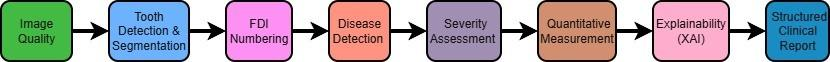
\includegraphics[width=\textwidth]{figures/phase2/p2_7_01_task_hierarchy.jpg}
\caption[Task hierarchy for panoramic radiograph analysis]{Task hierarchy for panoramic dental
radiograph analysis, adapted from the project's companion survey (Phase 2 report, Figure 7.1).}
\label{fig:taskhier}
\end{figure}
